%\documentclass[]{beamer}
\documentclass[handout]{beamer}
%\usepackage[dvips]{color}
\usepackage{graphicx}
\usepackage{amsmath,amssymb,array,comment,eucal}
\newcommand{\e}{\mathbf{e}}
\renewcommand{\P}{\mathbf{P}}
\newcommand{\F}{\mathbf{F}}
\newcommand{\R}{\textsf{R}}
\newcommand{\mat}[1] {\mathbf{#1}}
%\newcommand{\ind}{\mathrel{\mathop{\sim}\limits^{\mathit{ind}}}}
%\newcommand{\iid}{\mathrel{\mathop{\sim}\limits^{\mathit{iid}}}}
\newcommand{\E}{\textsf{E}}
\newcommand{\SE}{\textsf{SE}}
\newcommand{\SSE}{\textsf{SSE}}
\newcommand{\RSS}{\textsf{RSS}}
\newcommand{\FSS}{\textsf{FSS}}
\renewcommand{\SS}{\textsf{SS}}
\newcommand{\MSE}{\textsf{MSE}}
\newcommand{\SSR}{\textsf{SSR}}
\newcommand{\Be}{\textsf{Beta}}
\newcommand{\St}{\textsf{St}}
%\newcommand{\C}{\textsf{C}}
\newcommand{\GDP}{\textsf{GDP}}
\newcommand{\NcSt}{\textsf{NcSt}}
\newcommand{\Bin}{\textsf{Bin}}
\newcommand{\NB}{\textsf{NegBin}}
\renewcommand{\NG}{\textsf{NG}}
\newcommand{\N}{\textsf{N}}
\newcommand{\Ber}{\textsf{Ber}}
\newcommand{\Poi}{\text{Poi}}
\newcommand{\Gam}{\textsf{Gamma}}
\newcommand{\BB}{\textsf{BB}}
\newcommand{\Gm}{\textsf{G}}
\newcommand{\Un}{\textsf{Unif}}
\newcommand{\Ex}{\textsf{Exp}}
\newcommand{\DE}{\textsf{DE}}
\newcommand{\tr}{\textsf{tr}}
\newcommand{\cF}{{\cal{F}}}
\newcommand{\cL}{{\cal{L}}}
\newcommand{\cI}{{\cal{I}}}
\newcommand{\cB}{{\cal{B}}}
\newcommand{\cP}{{\cal{P}}}
\newcommand{\bbR}{\mathbb{R}}
\newcommand{\bbN}{\mathbb{N}}
\newcommand{\pperp}{\mathrel{{\rlap{$\,\perp$}\perp\,\,}}}
\newcommand{\OFP}{(\Omega,\cF, \P)}
\newcommand{\eps}{\boldsymbol{\epsilon}}
\newcommand{\1}{\mathbf{1}_n}
\newcommand{\gap}{\vspace{8mm}}
\newcommand{\ind}{\mathrel{\mathop{\sim}\limits^{\rm ind}}}
\newcommand{\simiid}{\ensuremath{\mathrel{\mathop{\sim}\limits^{\rm
iid}}}}
\newcommand{\eqindis}{\ensuremath{\mathrel{\mathop{=}\limits^{\rm D}}}}
\newcommand{\iid}{\textit{i.i.d.}}
\newcommand{\SSZ}{S_{zz}}
\newcommand{\SZW}{S_{zw}}
\newcommand{\Var}{\textsf{Var}}
\newcommand{\corr}{\textsf{corr}}
\newcommand{\diag}{\textsf{diag}}
\newcommand{\var}{\textsf{var}}
\newcommand{\Cov}{\textsf{Cov}}
\newcommand{\Sam}{{\cal S}}
\def\H{\mathbf{H}}
\newcommand{\I}{\mathbf{I}}
\newcommand{\Y}{\mathbf{Y}}
\newcommand{\tY}{\tilde{\mathbf{Y}}}
\newcommand{\Yhat}{\hat{\mathbf{Y}}}
\newcommand{\Yobs}{\mathbf{Y}_{{\cal S}}}
\newcommand{\barYobs}{\bar{Y}_{{\cal S}}}
\newcommand{\barYmiss}{\bar{Y}_{{\cal S}^c}}
\def\bv{\mathbf{b}}
\def\X{\mathbf{X}}
\def\tX{\tilde{\mathbf{X}}}
\def\x{\mathbf{x}}
\def\xbar{\bar{\mathbf{x}}}
\def\Xbar{\bar{\mathbf{X}}}
\def\Xg{\mathbf{X}_{\boldsymbol{\gamma}}}
\def\Ybar{\bar{\Y}}
\def\ybar{\bar{y}}
\def\y{\mathbf{y}}
\def\Yf{\mathbf{Y_f}}
\def\W{\mathbf{W}}
\def\L{\mathbf{L}}
\def\w{\mathbf{w}}
\def\U{\mathbf{U}}
\def\V{\mathbf{V}}
\def\Q{\mathbf{Q}}
\def\Z{\mathbf{Z}}
\def\z{\mathbf{z}}
\def\v{\mathbf{v}}
\def\u{\mathbf{u}}

\def\zero{\mathbf{0}}
\def\one{\mathbf{1}}
\newcommand{\taub}{\boldsymbol{\tau}}
\newcommand{\betav}{\boldsymbol{\beta}}
\newcommand{\alphav}{\boldsymbol{\alpha}}
\newcommand{\A}{\mathbf{A}}
\def\a{\mathbf{a}}
\def\K{\mathbf{K}}
\newcommand{\B}{\mathbf{B}}
\def\b{\boldsymbol{\beta}}
\def\bhat{\hat{\boldsymbol{\beta}}}
\def\btilde{\tilde{\boldsymbol{\beta}}}
\def\tb{\tilde{\boldsymbol{\beta}}}
\def\bg{\boldsymbol{\beta_\gamma}}
\def\bgnot{\boldsymbol{\beta_{(-\gamma)}}}
\def\mub{\boldsymbol{\mu}}
\def\tmub{\tilde{\boldsymbol{\mu}}}
\def\muhat{\hat{\boldsymbol{\mu}}}
\def\t{\boldsymbol{\theta}}
\def\tk{\boldsymbol{\theta}_k}
\def\tj{\boldsymbol{\theta}_j}
\def\Mk{\boldsymbol{{\cal M}}_k}
\def\M{\boldsymbol{{\cal M}}}
\def\Mj{\boldsymbol{{\cal M}}_j}
\def\Mi{\boldsymbol{{\cal M}}_i}
\def\Mg{{\boldsymbol{{\cal M}_\gamma}}}
\def\Mnull{\boldsymbol{{\cal M}}_{N}}
\def\gMPM{\boldsymbol{\gamma}_{\text{MPM}}}
\def\gHPM{\boldsymbol{\gamma}_{\text{HPM}}}
\def\Mfull{\boldsymbol{{\cal M}}_{F}}
\def\tg{\boldsymbol{\theta}_{\boldsymbol{\gamma}}}
\def\g{\boldsymbol{\gamma}}
\def\eg{\boldsymbol{\eta}_{\boldsymbol{\gamma}}}
\def\G{\mathbf{G}}
\def\cM{\cal M}
\def\D{\Delta}
\def \shat{{\hat{\sigma}}^2}
\def\uv{\mathbf{u}}
\def\l {\lambda}
\def\d{\delta}
\def\Sigmab{\boldsymbol{\Sigma}}
\def\Lambdab{\boldsymbol{\Lambda}}
\def\lambdab{\boldsymbol{\lambda}}
\def\Mg{{\cal M}_\gamma}
\def\S{{\cal{S}}}
\def\qg{p_{\boldsymbol{\gamma}}}
\def\pg{p_{\boldsymbol{\gamma}}}
\def\t{\boldsymbol{\theta}}  
\def\T{\boldsymbol{\Theta}}  
\usepackage{verbatim}

\usetheme{Warsaw}
\title{Checking Assumptions}
\subtitle{Merlise Clyde}
\author{STA721 Linear Models}
\institute{Duke University}
\date{October 8, 2012}
\logo{duke.eps}

\begin{document}
\maketitle

%\section{Models}
\begin{frame} \frametitle{ Linear Model}
Linear Model:
 $$ \Y = \mub + \eps $$ \pause
Assumptions: \pause
\begin{eqnarray*}
   \mub \in C(\X) & \Leftrightarrow & \mub = \X \b \pause \\
   \eps  & \sim &  \N(\zero_n, \sigma^2 \I_n) \pause
\end{eqnarray*}
Focus on 
\begin{itemize}
\item Wrong mean for a case or cases \pause \\
\item Wrong distribution for $\eps$  \\
\item Cases that influence the mean \pause
\end{itemize}
If $\mu_i \neq \x_i^T\b$ then expected value of $e_i = Y_i -\hat{Y}_i$
is not zero; 
\end{frame}

\begin{frame} \frametitle{Standardized residuals}
standardized residuals $$r_i = e_i/\sqrt{\sigma^2(1 - h_{ii})}$$

\begin{itemize}
%\item Under correct model have mean 0 and scale 1
%\item Use estimate of $\sigma^2$
\item The distribution of $r_$ is not a $t$
\item if $h_{ii}$ (leverage) is close to 1, then $\hat{Y}_i$ is close to
  $Y_i$ so $e_i$ is approximately 0
\item Variance is also almost 0, so standardize value may not flag ``outliers''
\end{itemize}

\end{frame}

\end{document}
  \begin{frame}
    \frametitle{Predicted Residuals}
Estimates without Case (i):

\begin{eqnarray*}
  \bhat_{(i)} & = & (\X_{(i)}^T\X_{(i)})^{-1 }\X_{(i)}^T \Y_{(i)}  \pause \\
 & = & \bhat - \frac{ (\X^T\X)^{-1} \x_i e_i}{ 1 - h_{ii}}   \pause
\end{eqnarray*}
 Predicted residual
$$ e_{(i)} = y_i - \x_i^T \bhat{(i)} = \frac{e_i}{1 - h_{ii}}$$
 \pause
with variance
$$\var(e_{(i)}) = \frac{\sigma^2}{1 - h_{ii}}$$
 \pause
Standardized predicted residual is 
$$\frac{e_{(i)}}{\sqrt{\var(e_{(i)})}}  = \frac{e_i/(1 -
  h_{ii})}{\sigma/\sqrt{1 - h_{ii}}} = \frac{e_i}{\sigma \sqrt{1 -
    h_{ii}} } 
$$ \pause
Can show that these are the same as standardized residual!
  \end{frame}
  \begin{frame}
    \frametitle{External estimate of $\sigma^2$}
    Estimate $\shat_{(i)}$ using data with case $i$ deleted  \pause
    \begin{eqnarray*}
\SSE_{(i)} & = &  \SSE - \frac{e_i^2}{1 - h_{ii}}  \pause \\
\shat_{(i)} = \MSE_{(i)} & = &  \frac{\SSE_{(i)}}{n - p - 1}  \pause\\
    \end{eqnarray*}
Externally Standardized residuals  \pause
$$t_i = \frac{e_{(i)}}{\sqrt{\shat_{(i)}/(1 - h_{ii})}}  =  \frac{y_i
  - \x_i^T \bhat_{(i)}} {\sqrt{\shat_{(i)}/(1 - h_{ii})}} \pause =  r_i \left(
\frac{ n - p - 1}{n - p - r_i^2}\right)^{1/2}$$  \pause



May still miss extreme points with high leverage, but will pick up unusual $y_i$s
  \end{frame}
  \begin{frame}
    \frametitle{Distribution of Externally Studentized Residual}
\vspace{-48pt}
    $$t_i = \frac{e_{(i)}}{\sqrt{\shat_{(i)}/(1 - h_{ii})}}  =  \frac{y_i
  - \x_i^T \bhat_{(i)}} {\sqrt{\shat_{(i)}/(1 - h_{ii})}}  \sim \St(n
- p - 1)$$

\vfill

  \end{frame}

  \begin{frame}
    \frametitle{Outlier Test}
    H$_0$: $\mu_i = \x_i^T \b$  versus H$_a$: $\mu_i = \x_i^T\b +
    \alpha_i$  \pause
    \begin{itemize}
    \item  Show that t-test for testing H$_0$: $\alpha_i = 0$ is equal
      to $t_i$   \pause
  \item if p-value is
small declare the $i$th case to be an outlier:  $\E[Y_i]$ not given by
$\X \b$  but $\X\b + \delta_i \alpha_i$    \pause
\item Can extend to include multiple $\delta_i$ and $\delta_j$ to test
  that case $i$ and $j$ are both outliers \pause
\item Extreme case $\mub = \X\b + \I_n \alphav$  all points have their
  own mean!   \pause
\item Control for multiple testing  \pause
    \end{itemize}
  \end{frame}
  \begin{frame}
    \frametitle{Multiple Testing}
    look to see if the $\max |t_i|$ is larger than expected under the
    null \pause
    \begin{itemize}
    \item Need distribution of the max of Student $t$ random variables
      (simulate) \pause
\item Conservative is Bonferroni Correction:  For $n$ tests of size
  $\alpha$ the probability of falsely labeling at least one case as an
  outlier is no greater than $n \alpha$; e.g. with 21 cases and
  $\alpha = 0.05$, the probability is no greater than 1.05!
\pause
\item Adjust $\alpha^* = \alpha/n$ so that the probability of falsely
  labeling at least one point an outlier is $\alpha$
  $\alpha/n = .00238$
\pause
    \end{itemize}
  \end{frame}
  \begin{frame}
    \frametitle{Cook's Distance}
    Cook's Distance  measure of how much predictions change with $i$th
    case deleted  \pause
    \begin{eqnarray*}
D_i & =  &\frac{\| \Y_{(i)} - \Y \|^2}{ p \shat} = 
\frac{ (\bhat_{(i)} - \bhat)^T \X^T\X (\bhat_{(i)} - \bhat) }{ p
  \shat}  \pause \\
& = & \frac{r_i^2}{p} \frac{h_{ii}}{ 1 - h_{ii}}  \pause
    \end{eqnarray*}
Flag cases where $D_i > 1$ or large relative to other cases
 \pause

\vspace{18pt}
Influential Cases
  \end{frame}
  \begin{frame}
   \frametitle{Stackloss Data}
\vspace{-24pt}
    \centerline{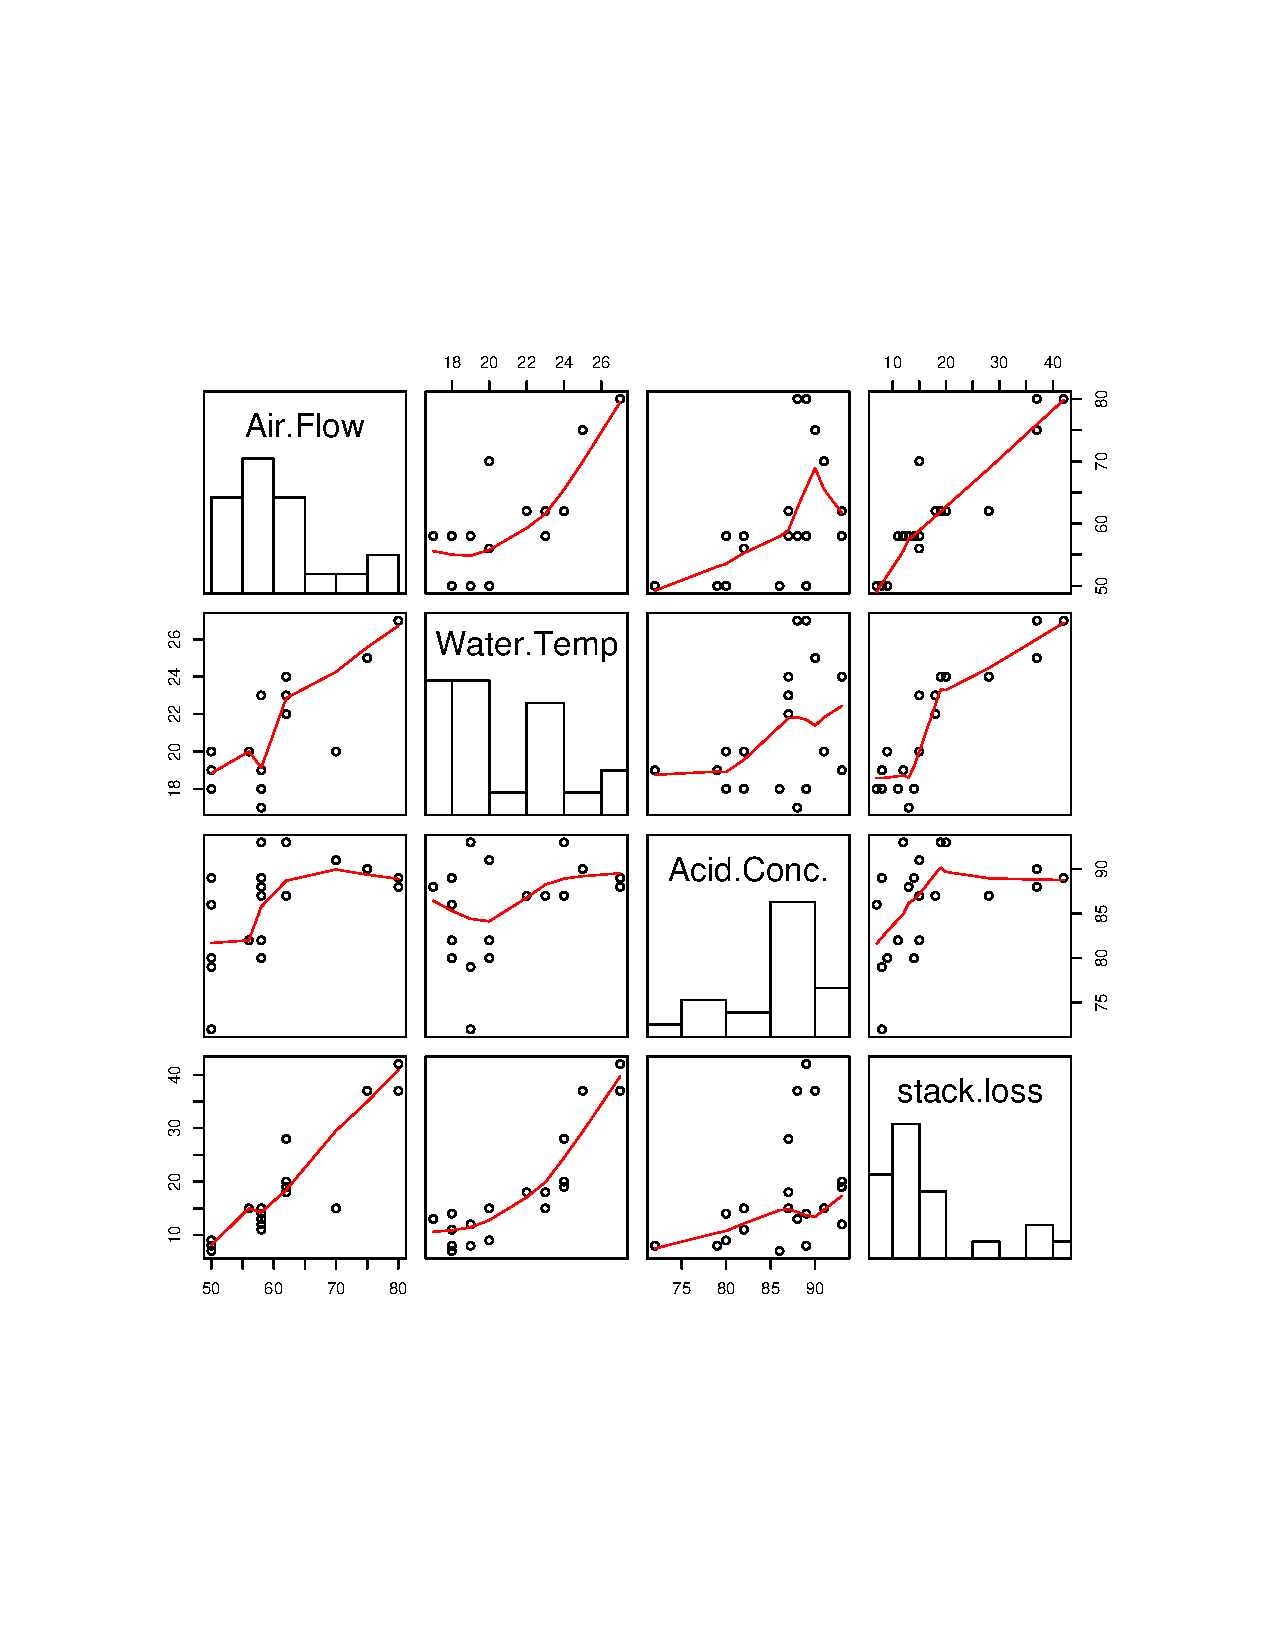
\includegraphics[height=4in]{stackloss-pair}}
  \end{frame}
  \begin{frame}
    \frametitle{Stackloss Added Variable Plot}
    \centerline{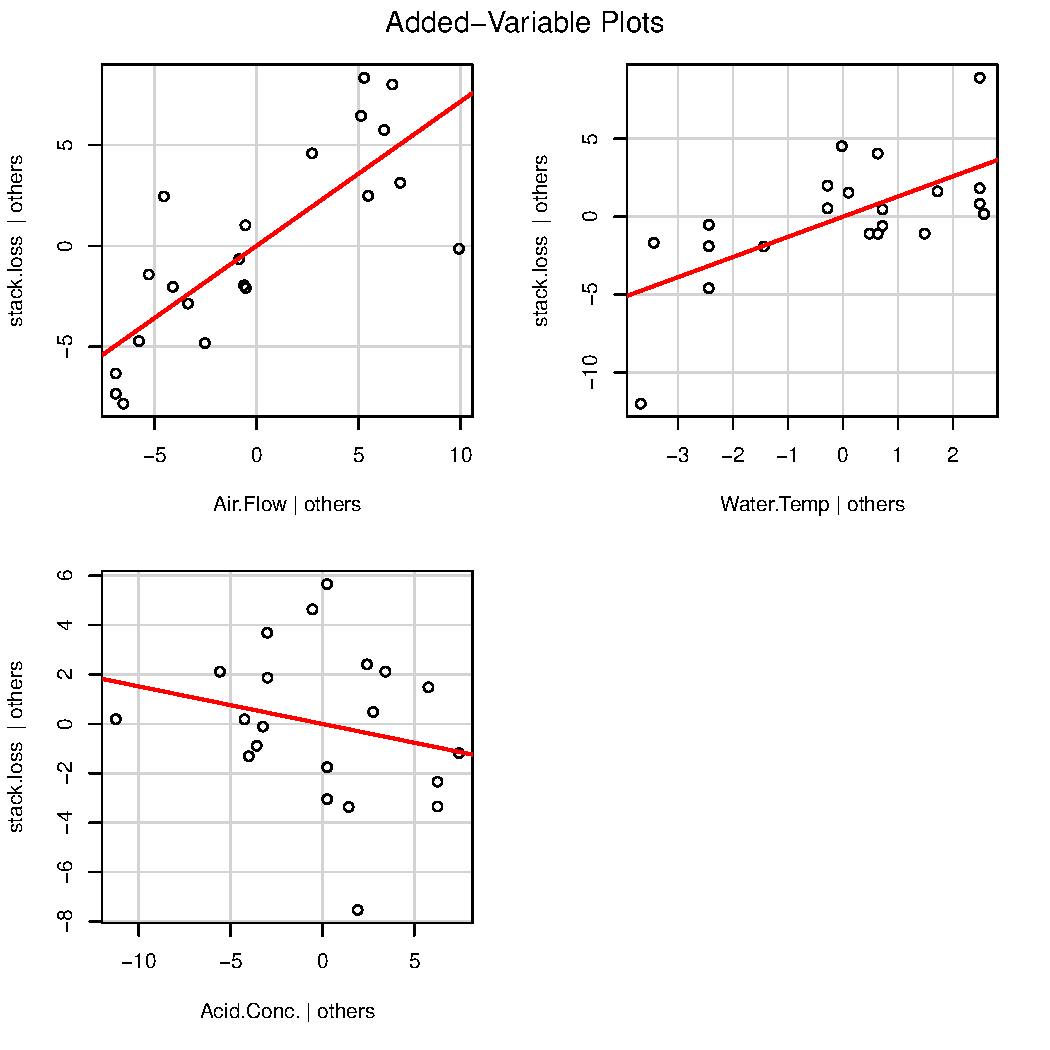
\includegraphics[height=3.5in]{stackloss-avp}}
  \end{frame}
  \begin{frame}
    \frametitle{Stackloss Data Again}
    \centerline{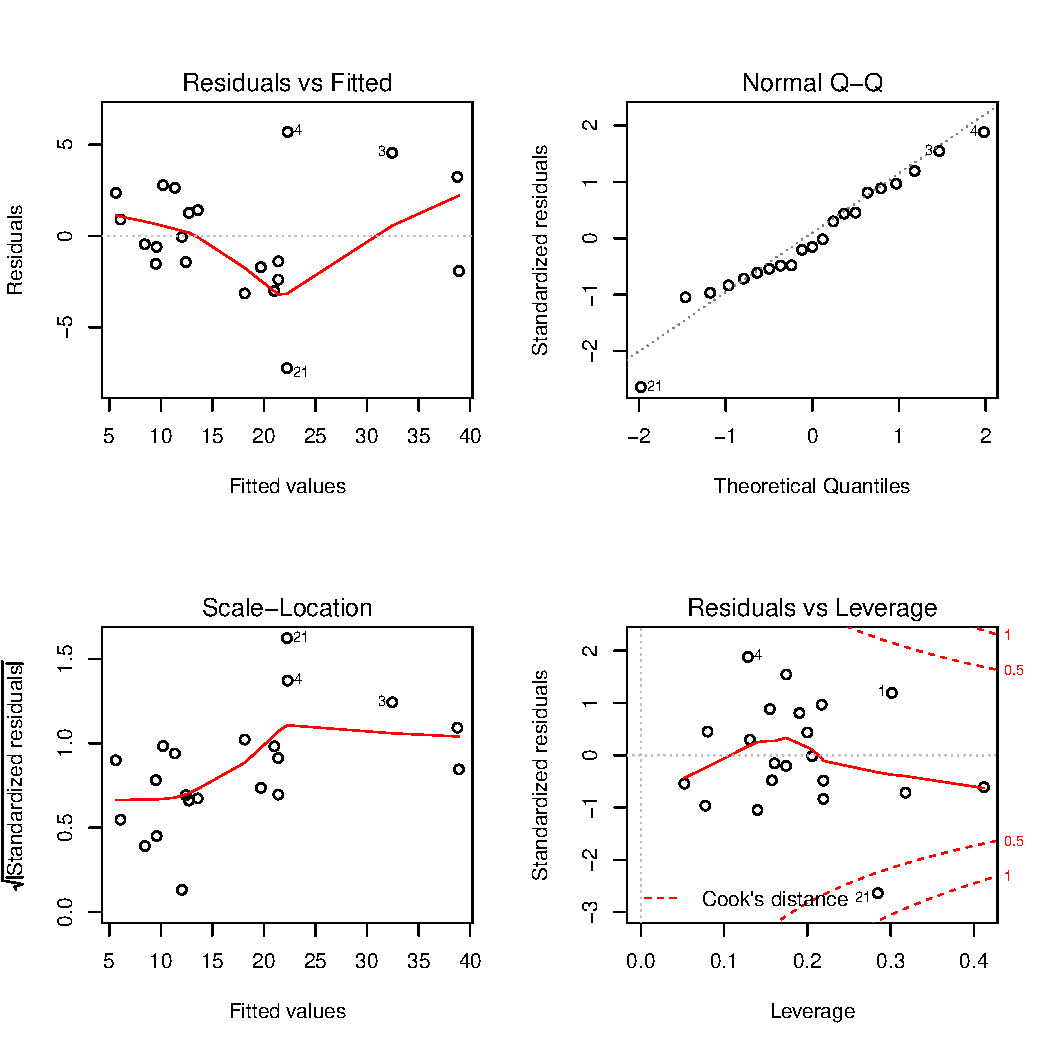
\includegraphics[height=3.5in]{stackloss-resid}}
  \end{frame}
  \begin{frame}
    \frametitle{Case 21}
    \begin{itemize}
    \item Leverage $0.285$  (compare to $p/n = .19$ ) \pause
\item p-value $t_{21}$ is $0.0042$ \pause
\item Bonferroni adjusted p-value is $0.0024$ \pause
\item Cooks' Distance $.69$   \pause
\item Other points?  Masking?  \pause
\item Refit without Case 21 \pause
    \end{itemize}
Other analyses have suggested that cases (1, 2, 3, 4, 21) are outliers
  \end{frame}
  \begin{frame}
   \frametitle{Stackloss Data}
\vspace{-24pt}
    \centerline{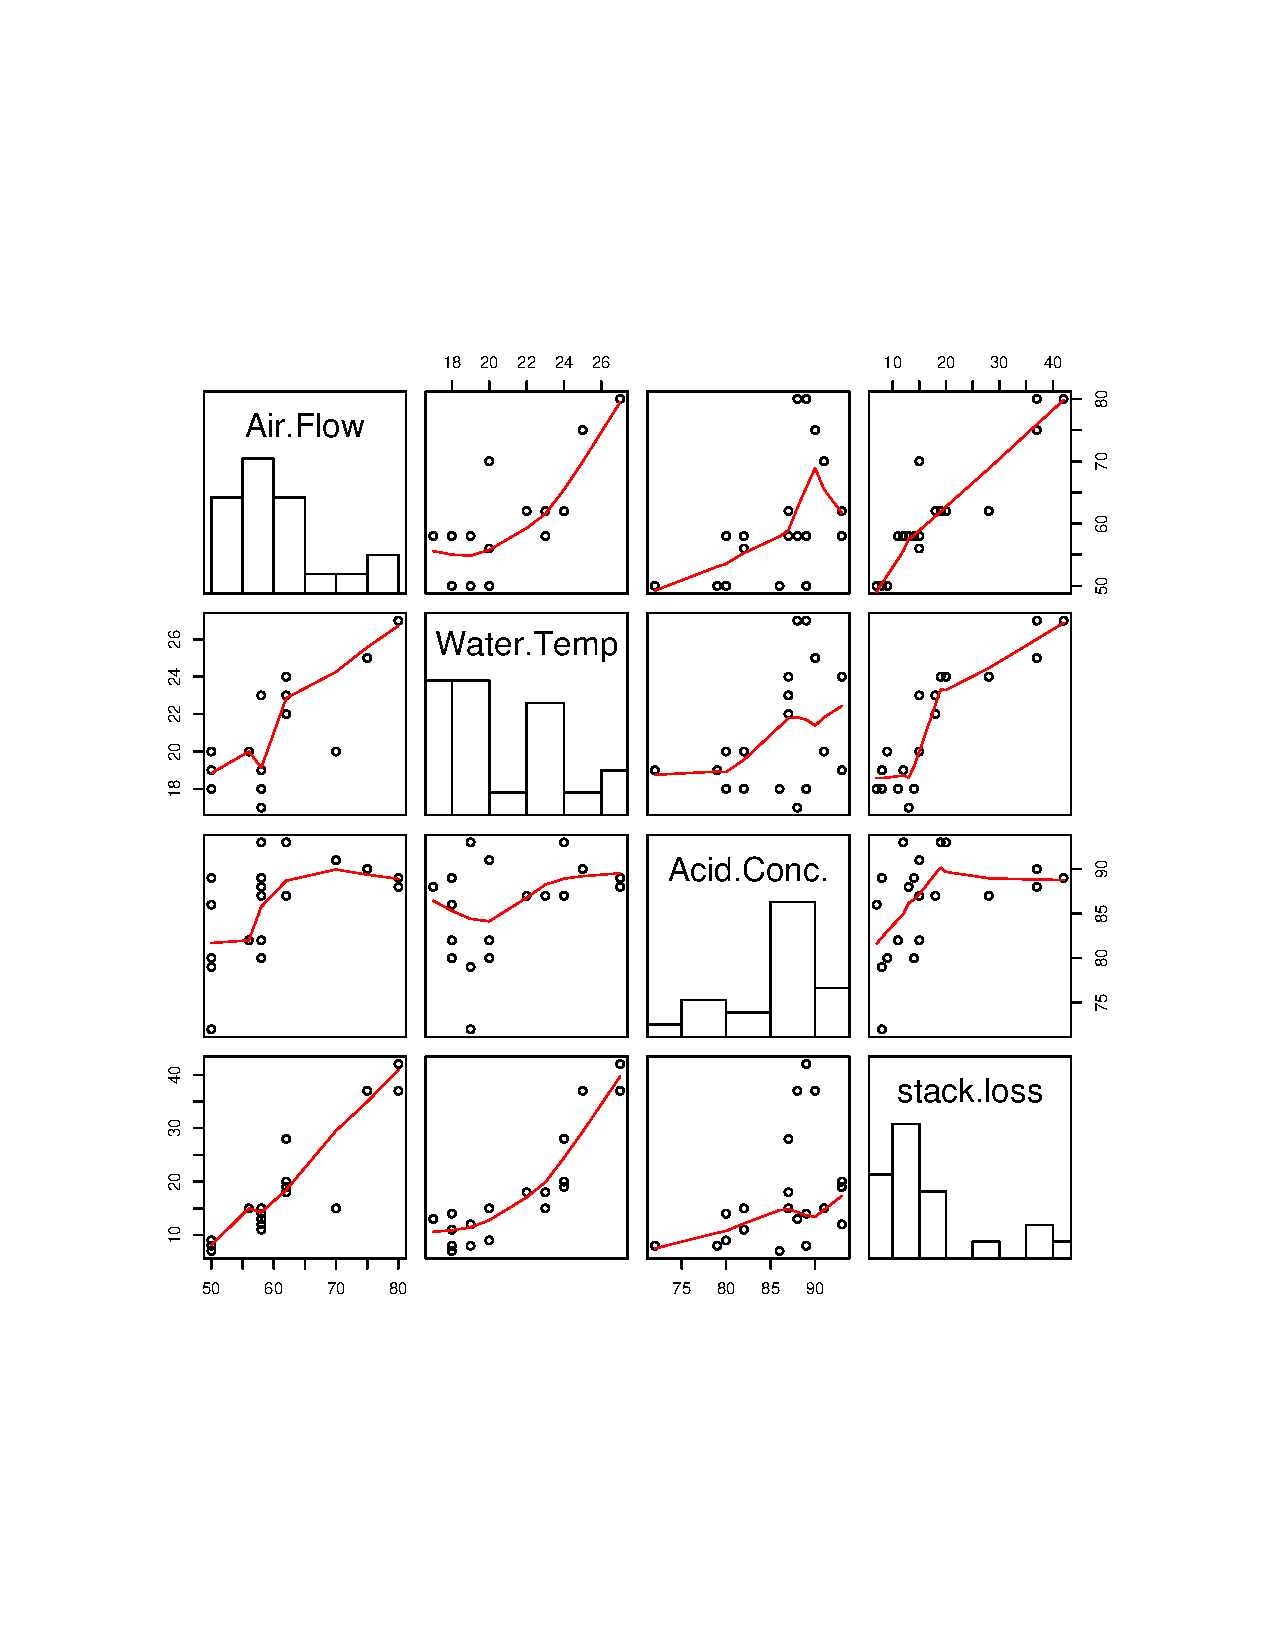
\includegraphics[height=4in]{stackloss-pair}}
Conclusion?  \pause non-linearity?
  \end{frame}

  \begin{frame}
    \frametitle{Normality}
    Recall
    \begin{eqnarray*}
 \e & = &(\I - \P_\X) \Y \pause \\      
 & = & (\I - \P_\X)(\X \bhat + \eps)  \pause\\
 & = &  (\I - \P_\X)\eps  \pause
    \end{eqnarray*}
$$e_i = \epsilon_i - \sum_{j=1}^n h_{ij} \epsilon_j$$  \pause
Lyapunov CLT implies that  residuals will be approximately normal
(even for modest $n$), 
if the errors are not normal  \pause

\vfill

``Supernormality of residuals''
  \end{frame}
  \begin{frame}
    \frametitle{Q-Q Plots}
\begin{itemize}
\item Order $e_i$: $e_{(1)} \le e_{(2)} \ldots \le e_{(n)}$  sample
    order statistics or sample quantiles  \pause
\item Let $z_{(1)} \le z_{(2)} \ldots z_{(n)}$ denote the expected
  order statistics of a sample of size $n$ from a standard normal
  distribution ``theoretical quantiles''  \pause
\item If the $e_i$ are normal then $\E[e_{(i)}] = \sigma z_{(i)}$   \pause
\item Expect that points in a scatter plot of $e_{(i)}$ and $z_{(i)}$
  should be on a straight line.  \pause
\item Judgment call - use simulations to gain experience!
\end{itemize}
    
  \end{frame}

  \begin{frame}
    \frametitle{Animal Example}

\centerline{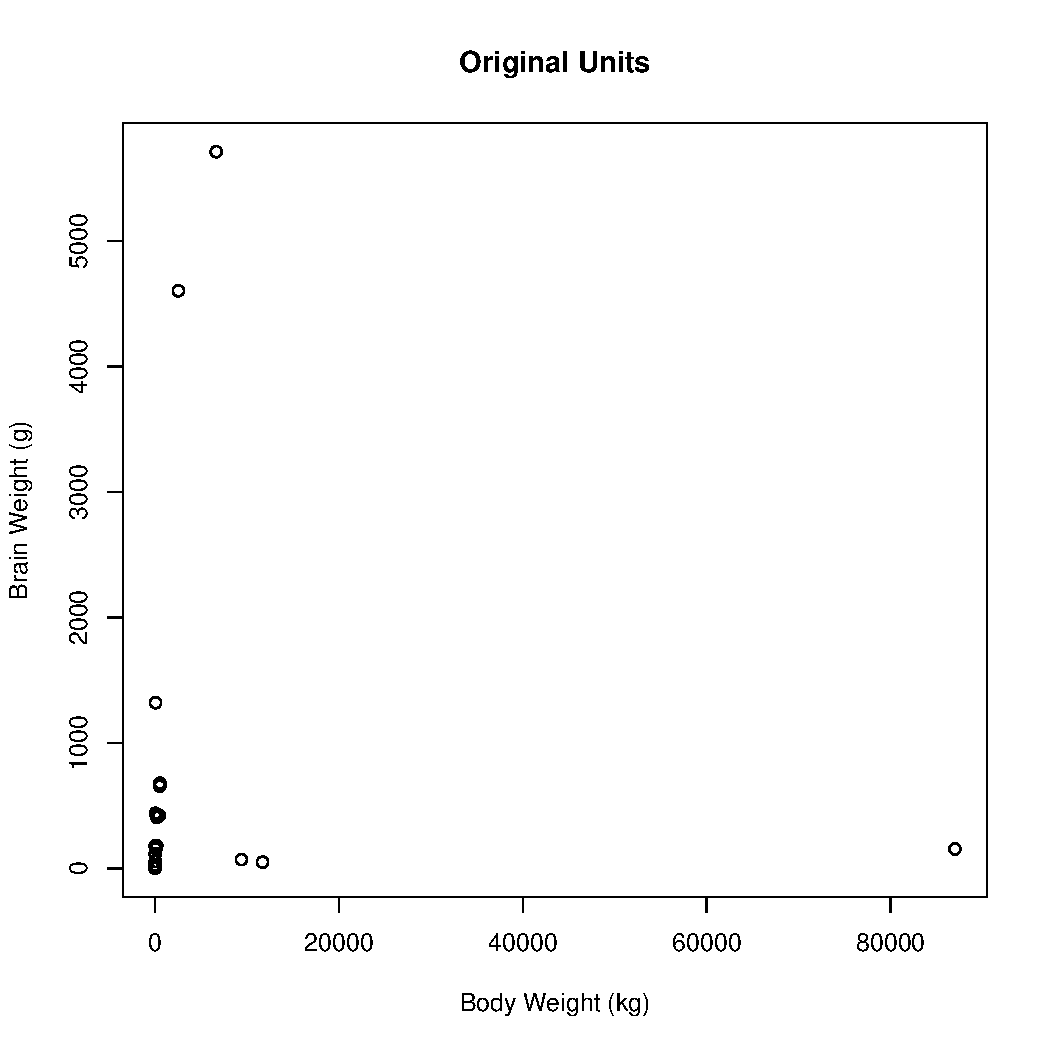
\includegraphics[height=3in]{brain}}
  \end{frame}

  \begin{frame}
    \frametitle{Residual Plots}

\centerline{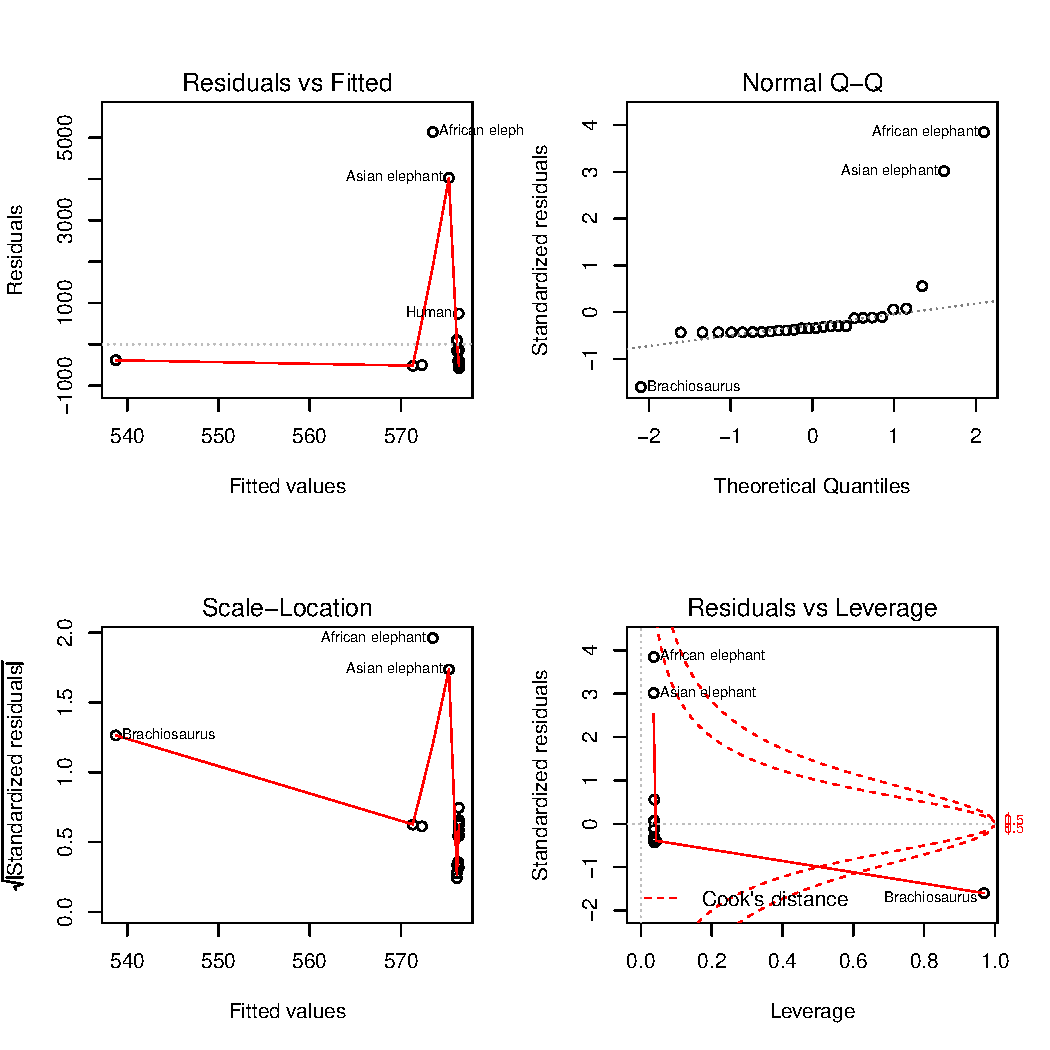
\includegraphics[height=3in]{brains-resid}}
  \end{frame}


  \begin{frame}
    \frametitle{Box-Cox Transformation}
    Box and Cox (1964) suggested a family of power transformations for
    $Y > 0$  \pause
$$
U(\Y, \lambda) =  Y^{(\lambda)} = \left\{
   \begin{array}{ll}
     \frac{(Y^\lambda -1)}{\lambda} & \lambda \neq 0 \\
 \log(Y) & \lambda = 0
   \end{array} \right.
$$  \pause

\begin{itemize}
\item Estimate $\lambda$ by maximum Likelihood  \pause
$$\cL(\lambda, \b, \sigma^2) \propto \prod f(y_i \mid \lambda, \b,
\sigma^2)$$

\item  $U(\Y, \lambda) = Y^{(\lambda)} \sim \N(\X\b, \sigma^2)$
  \pause
\item Jacobian term is $\prod_i y_i^{\lambda - 1}$ for all $\lambda$  \pause
\item Profile Likelihood based on substituting MLE $\b$ and $\sigma^2$
  for each value of $\lambda$ is 
$$\log(\cL(\lambda) \propto (\lambda -1)
\sum_i \log(Y_i) - \frac{n}{2} \log(\SSE (\lambda))$$
\end{itemize}

  \end{frame}
  \begin{frame}
    \frametitle{ Profile Likelihood}

\centerline{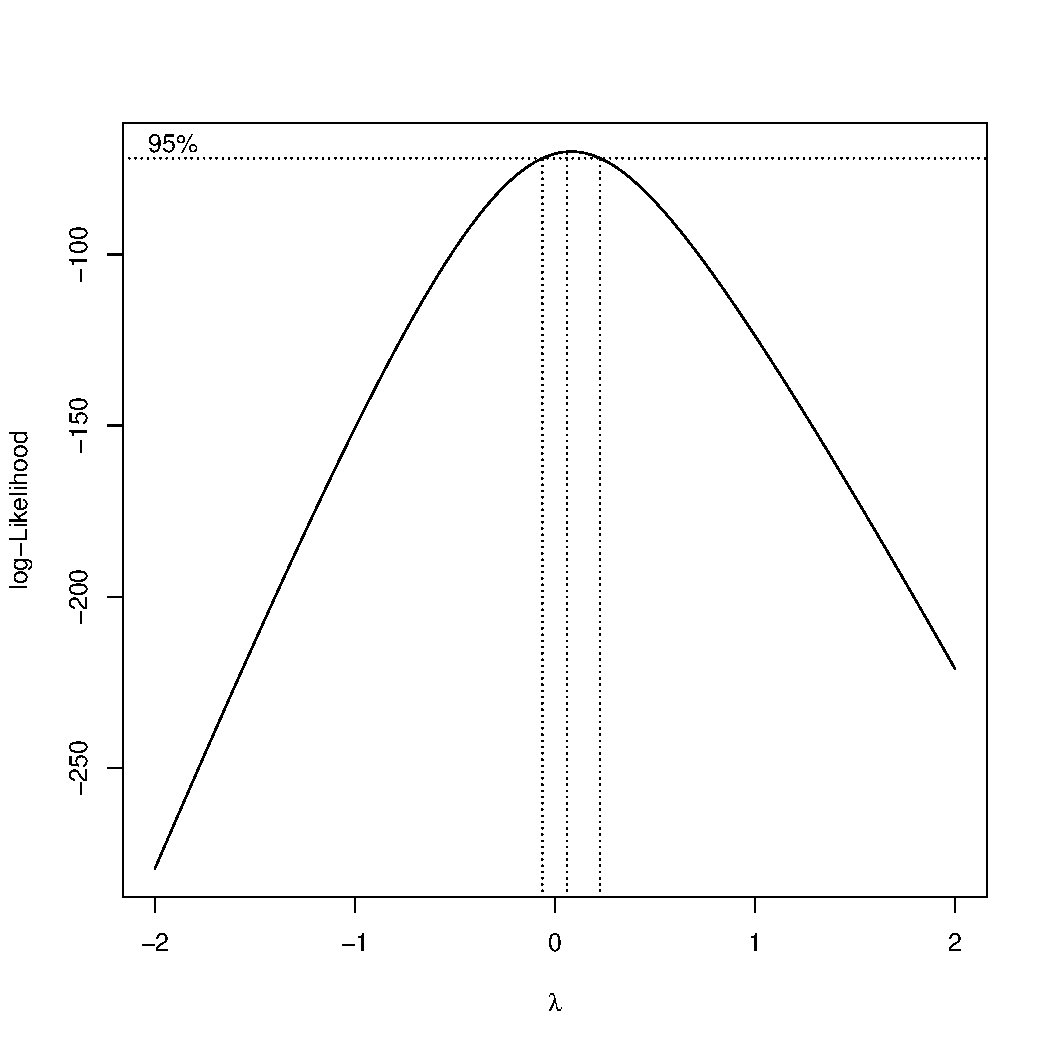
\includegraphics[height=3in]{brains-BC}}
  \end{frame}

  \begin{frame}
    \frametitle{ Residuals After Transformation of Response}

\centerline{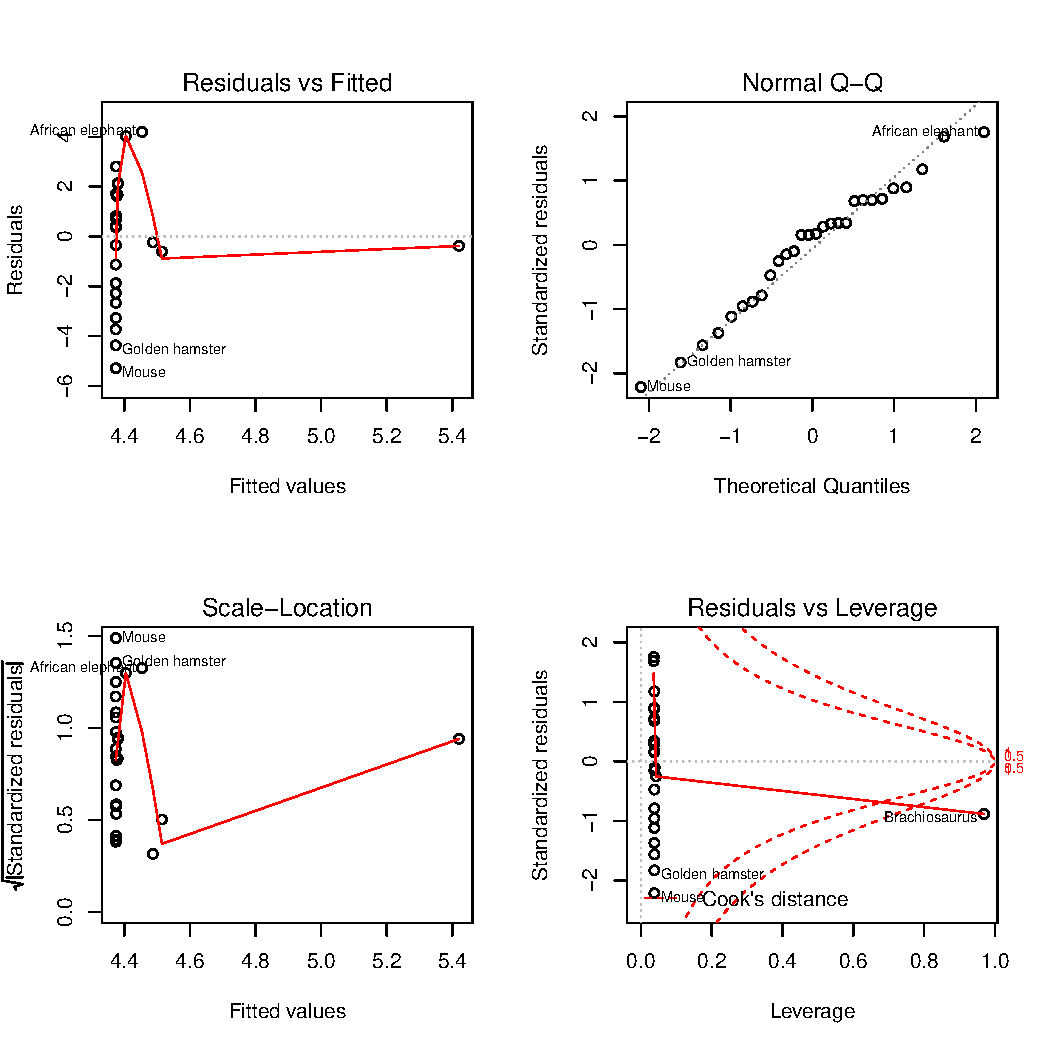
\includegraphics[height=3in]{brain-resid-logY}}

  \end{frame}
  \begin{frame}
    \frametitle{ Residuals After Transformation of Both}

\centerline{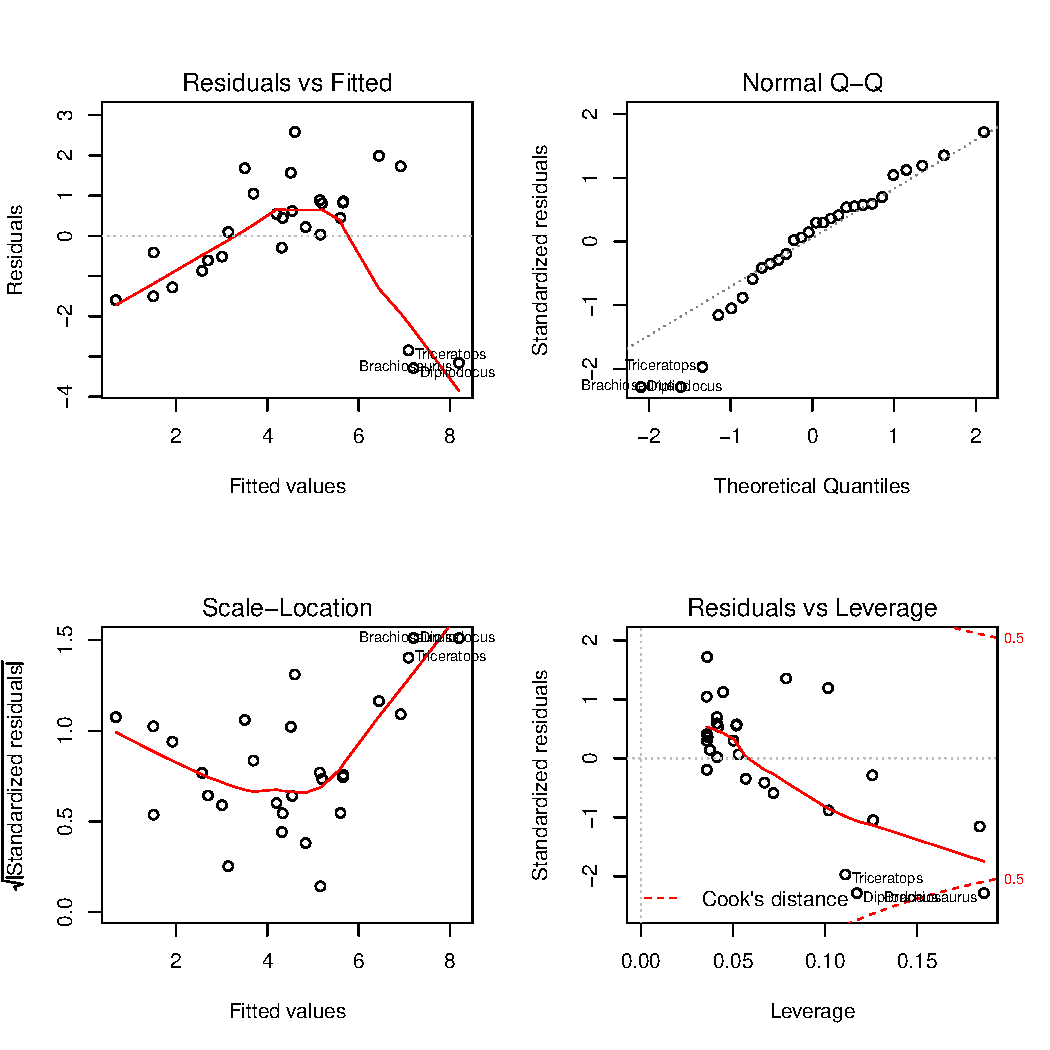
\includegraphics[height=3in]{brains-tran}}

  \end{frame}

 \begin{frame}
    \frametitle{ Transformed Data}

\centerline{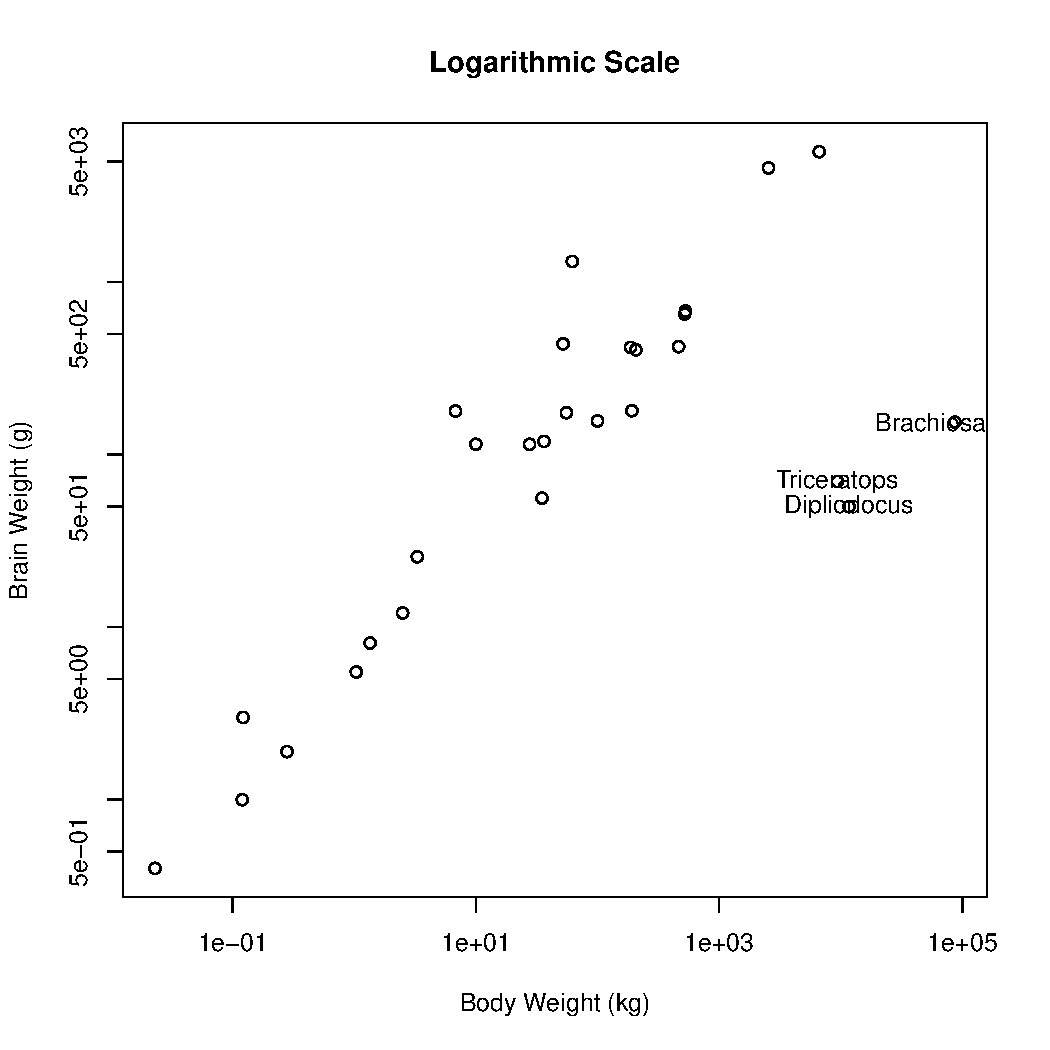
\includegraphics[height=3in]{brain-log}}

  \end{frame}

  \begin{frame}
    \frametitle{Test that Dinos are Outliers}
    \begin{table}[ht]
\begin{center}
\begin{tabular}{lrrrrrr}
  \hline
 & Res.Df & RSS & Df & Sum of Sq & F & Pr($>$F) \\ 
  \hline
1 & 23 & 12.12 &  &  &  &  \\ 
  2 & 26 & 60.99 & -3 & -48.87 & 30.92 & 0.0000 \\ 
   \hline
\end{tabular}
\end{center}
\pause
\begin{table}[ht]
\begin{center}
\begin{tabular}{rrrrr}
  \hline
 & Estimate & Std. Error & t value & Pr($>$$|$t$|$) \\ 
  \hline
(Intercept) & 2.1504 & 0.2006 & 10.72 & 0.0000 \\ 
  log(body) & 0.7523 & 0.0457 & 16.45 & 0.0000 \\ 
  Triceratops & -4.7839 & 0.7913 & -6.05 & 0.0000 \\ 
  Brachiosaurus & -5.6662 & 0.8328 & -6.80 & 0.0000 \\ 
  Dipliodocus & -5.2851 & 0.7949 & -6.65 & 0.0000 \\ 
   \hline
\end{tabular}
\end{center}
\end{table}
\pause
Dinosaurs come from a different population from mammals
\end{table}
  \end{frame}
  \begin{frame} \frametitle{To Remove or Not?}
    \begin{itemize}
    \item  For suspicious cases, check data sources for errors \pause
    \item  Check that points are not outliers because of wrong mean
      function or distributional assumptions  \pause
  \item Investigate need for transformations  (use EDA at several stages)
   \item Influential cases - report results with and without cases
     (results may change - are differences meaningful?)  \pause
   \item Outlier test - suggests alternative population for the case(s); if not
     influential may in keep analysis, but will inflate $\shat$ and
     interval estimates   \pause
   \item Document how you handle any case deletions - reproducibility! \pause
   \item Robust Regression Methods  \pause
    \end{itemize}
  \end{frame}

\end{document}


